\chapter{Background}
\label{background}

This chapter outlines background information about nutritional assessment using computer vision.
An overview of neural networks is explored, followed by a literature review of the subject area.
Analysis into evaluating the efficacy of CNNs is covered and finally a conclusion to the information gained.

\section{Introduction to Machine Learning}
In \parencite{MLANN}, machine learning is defined as "the question of how to
construct computer programs that automatically improve with experience".
Machine learning has blossomed in recent years with applications across multiple
domains using vastly different paradigms and technologies. 
Some of the different approaches used in machine learning are: Artificial Neural Networks, Genetic Algorithms, Decision Tree Learning and Bayesian Learning \parencite{MLANN}.

There are many ways in which machine learning can be used in the modern world,
many of which are being utilised to great effect.
Some of these applications are image recognition, natural language
processing and many more.
These applications can be applied to many different domains such as security (face detection in airports) or object detection (autonomous driving).
\parencite{medical} carried out research into the area of using machine learning to aid diagnosis of medical conditions.
Machine learning algorithms could suggest possible diagnosis for medical professionals to interpret and therefore reduce the time spent diagnosing a patient's condition.
There may be fear that machine learning will start to take away many jobs
from
humans, but this may not be the case as in the example above as computers will only be aiding professionals.

One of the most exciting avenues in machine learning is computer
vision.
This is due to the application domains mentioned above. 
Computer vision is the process of extracting high-dimensional data from an image to produce useful information, which in terms of classification usually results in labelling. It can be used in many areas to improve our lives. As
mentioned earlier, autonomous cars are only possible when a machine can
determine what objects are around it. Computer Vision can allow a machine to
recognise medical conditions in an image such as breast cancer using mammography images \parencite{medical}. The applications are nearly limitless.

\section{Neural Computing}
The main area of my focus for this project is in
Artificial Neural Networks (ANN). This is because extensive research has been carried out into Convolutional Neural Networks (CNNs) which are based on ANNs.
\subsection*{Artificial Neural Networks}
An Artificial Neural Network is a bio-inspired system that is used to model the human brain in how it learns from experience.
The ANN uses this model to build a very complex web of connected units called
artificial neurons.
These neurons are connected by certain weights which determines the processing
capacity of the network and these weights are created by learning a
dataset.(reference Malachy)
An ANN has a set of inputs that take in a value, sometimes from network outputs
and produce a single result or classification.
While an ANN is bio-inspired from the human brain, there are many elements of
the brain that are not present in ANN and many new elements in ANN that are not
modeled from the human brain.

Before Convolution Neural Networks can be explored, which are vital to image
processing, the perceptron learning algorithm, the multi
layer perceptron, backpropogation must be analysed.

\tocless\subsubsection{Perceptron Learning - Artificial Neuron}
In our ANN, a perceptron is an artificial neuron.
It is called an artificial neuron because it is a bio-inspired neuron which models
a neuron in the human brain in terms of inputs and output.

In perceptron learning, we can take two inputs which are put towards an
activation function with a bias attached as seen in Figure \ref{fig:perceptron}.
These inputs are multiplied by the weights that connect the input to the
activation function and depending on the result, the activation function may
fire an output. These inputs are either 1 or -1.

\begin{figure}[h]
	\centering
     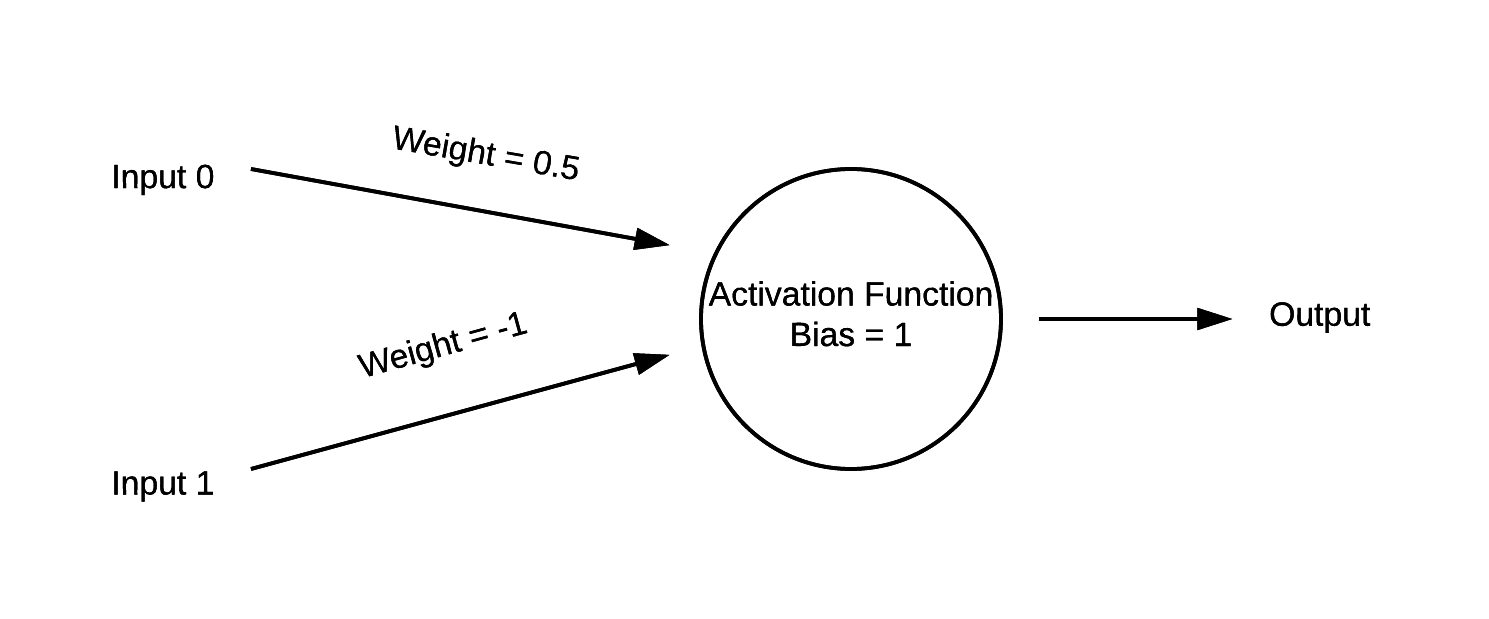
\includegraphics{Perceptron}
     \caption{Perceptron}
     \label{fig:perceptron}
\end{figure}

The Perceptron Training Rule is how weights are selected to produce the correct output during training.
As in \parencite{MLANN}, a common way to train a perceptron is to start with random weights and change them during training as per the training rule.
This rule follows the formula in Equation \ref{eqn:perceptron1}, where xi is the input and Equation \ref{eqn:perceptron2} is valid:
\begin{equation}\label{eqn:perceptron1}
    w_{i} \leftarrow w_{i} + \Delta w_{i}
\end{equation}

\begin{equation}\label{eqn:perceptron2}
    \Delta w_{i} = n(t-o)x_{i}
\end{equation}

In Equation \ref{eqn:perceptron2}, "t is the target output for the current training example, o is the output generated by the perceptron, and n is the positive constant called the learning rate" \parencite{MLANN}.
The output of a neuron is calculated using the activation function.
This Perceptron Training Rule assumes that there are two sets of instances, a
positive and negative set (class x and - in Figure \ref{fig:ls}), and that they are linearly separable, as in demonstrated in Figure \ref{fig:ls}. 

\begin{figure}[h]
	\centering
    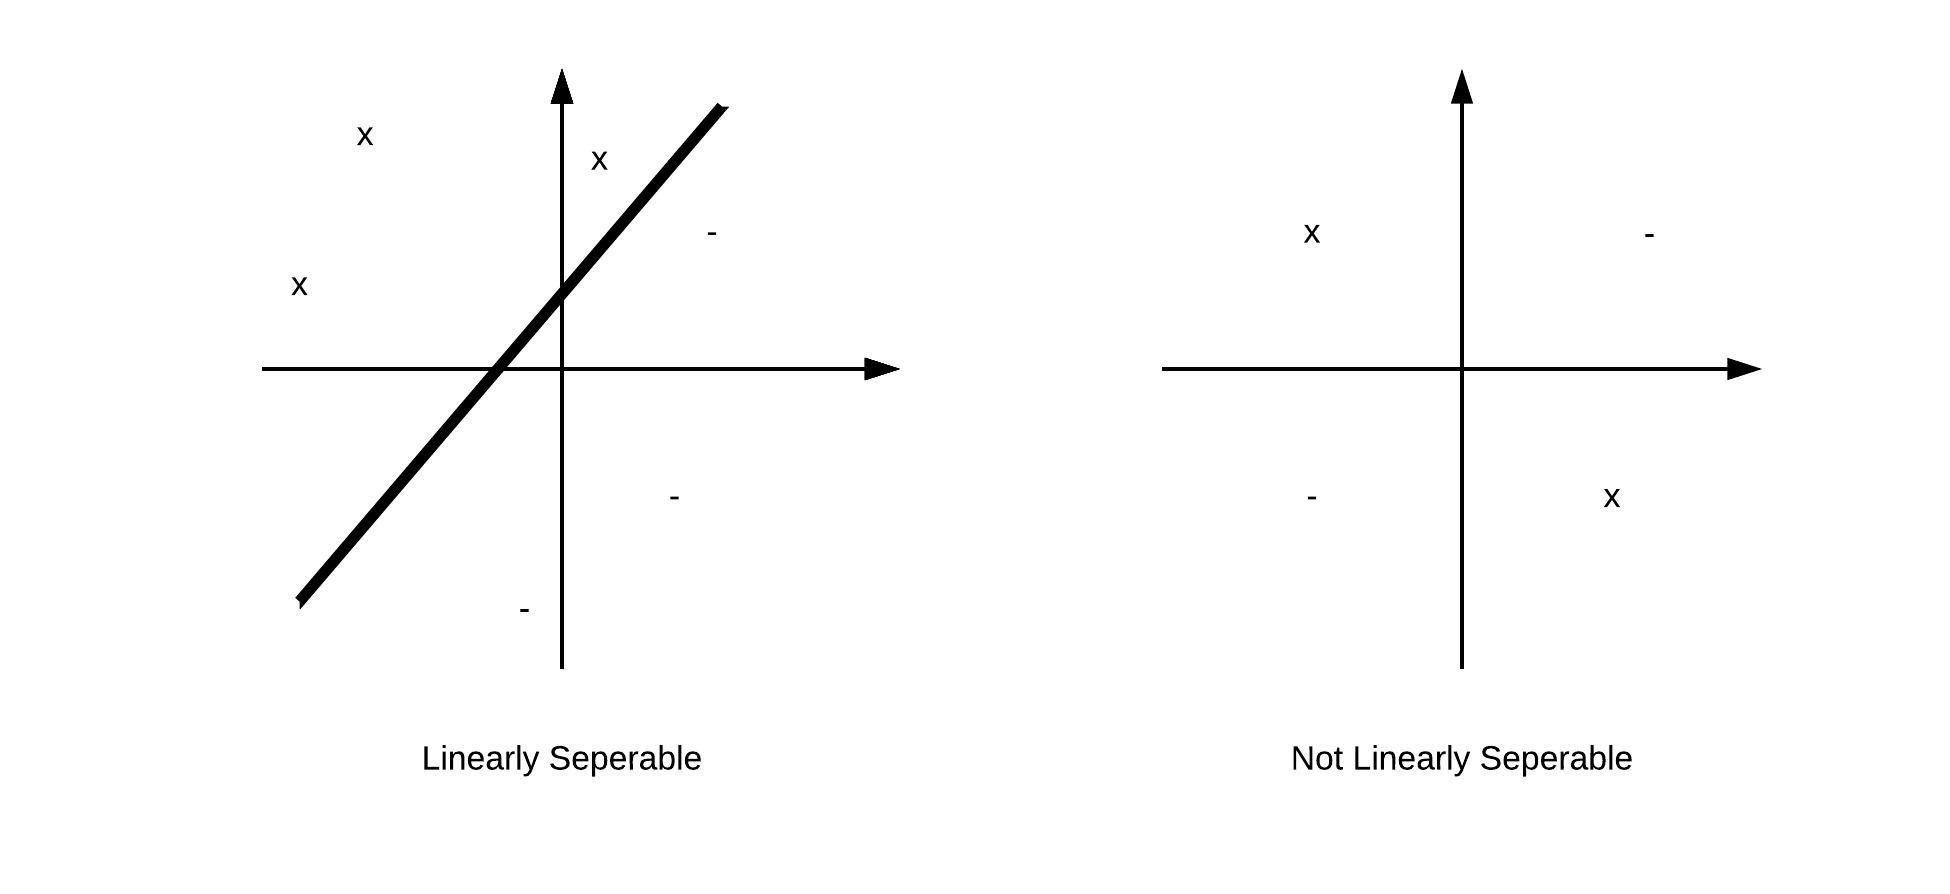
\includegraphics{LS}
     \caption{Linearly Separable, adapted from \parencite{MLANN}}
     \label{fig:ls}
\end{figure}

A perceptron is trained using supervised learning. When the perceptron
classifies a result, it is told if it is correct or not. If the result is
incorrect, weights are changed in value so that this error can be reduced
\parencite{AI}. 

There is one major problem with perceptron learning and that is, it can't solve
a problem if there is not a clear linear separation between the classes. There
is a way in which we can attempt to solve this, through the delta rule. The
delta rule utilises gradient descent to find the best weight for the training
samples \parencite{MLANN}. We will discuss gradient descent in the next section.

\tocless\subsubsection{Multi Layered Perceptron}
Multi-Layer Perceptrons (MLPs) are made up of multiple layers of perceptrons connected
together and are used to combat non-linearly separable classes.
While the delta rule can solve problems of non-linearity when there are two classes, MLPs can solve non-linearity when there are more than two classes.
Firstly, we have an input layer, followed by one or more hidden layers and then
finally an output layer.
Any ANN with more than three hidden layers is categorised as a deep neural network.

\begin{figure}[h]
	\centering
    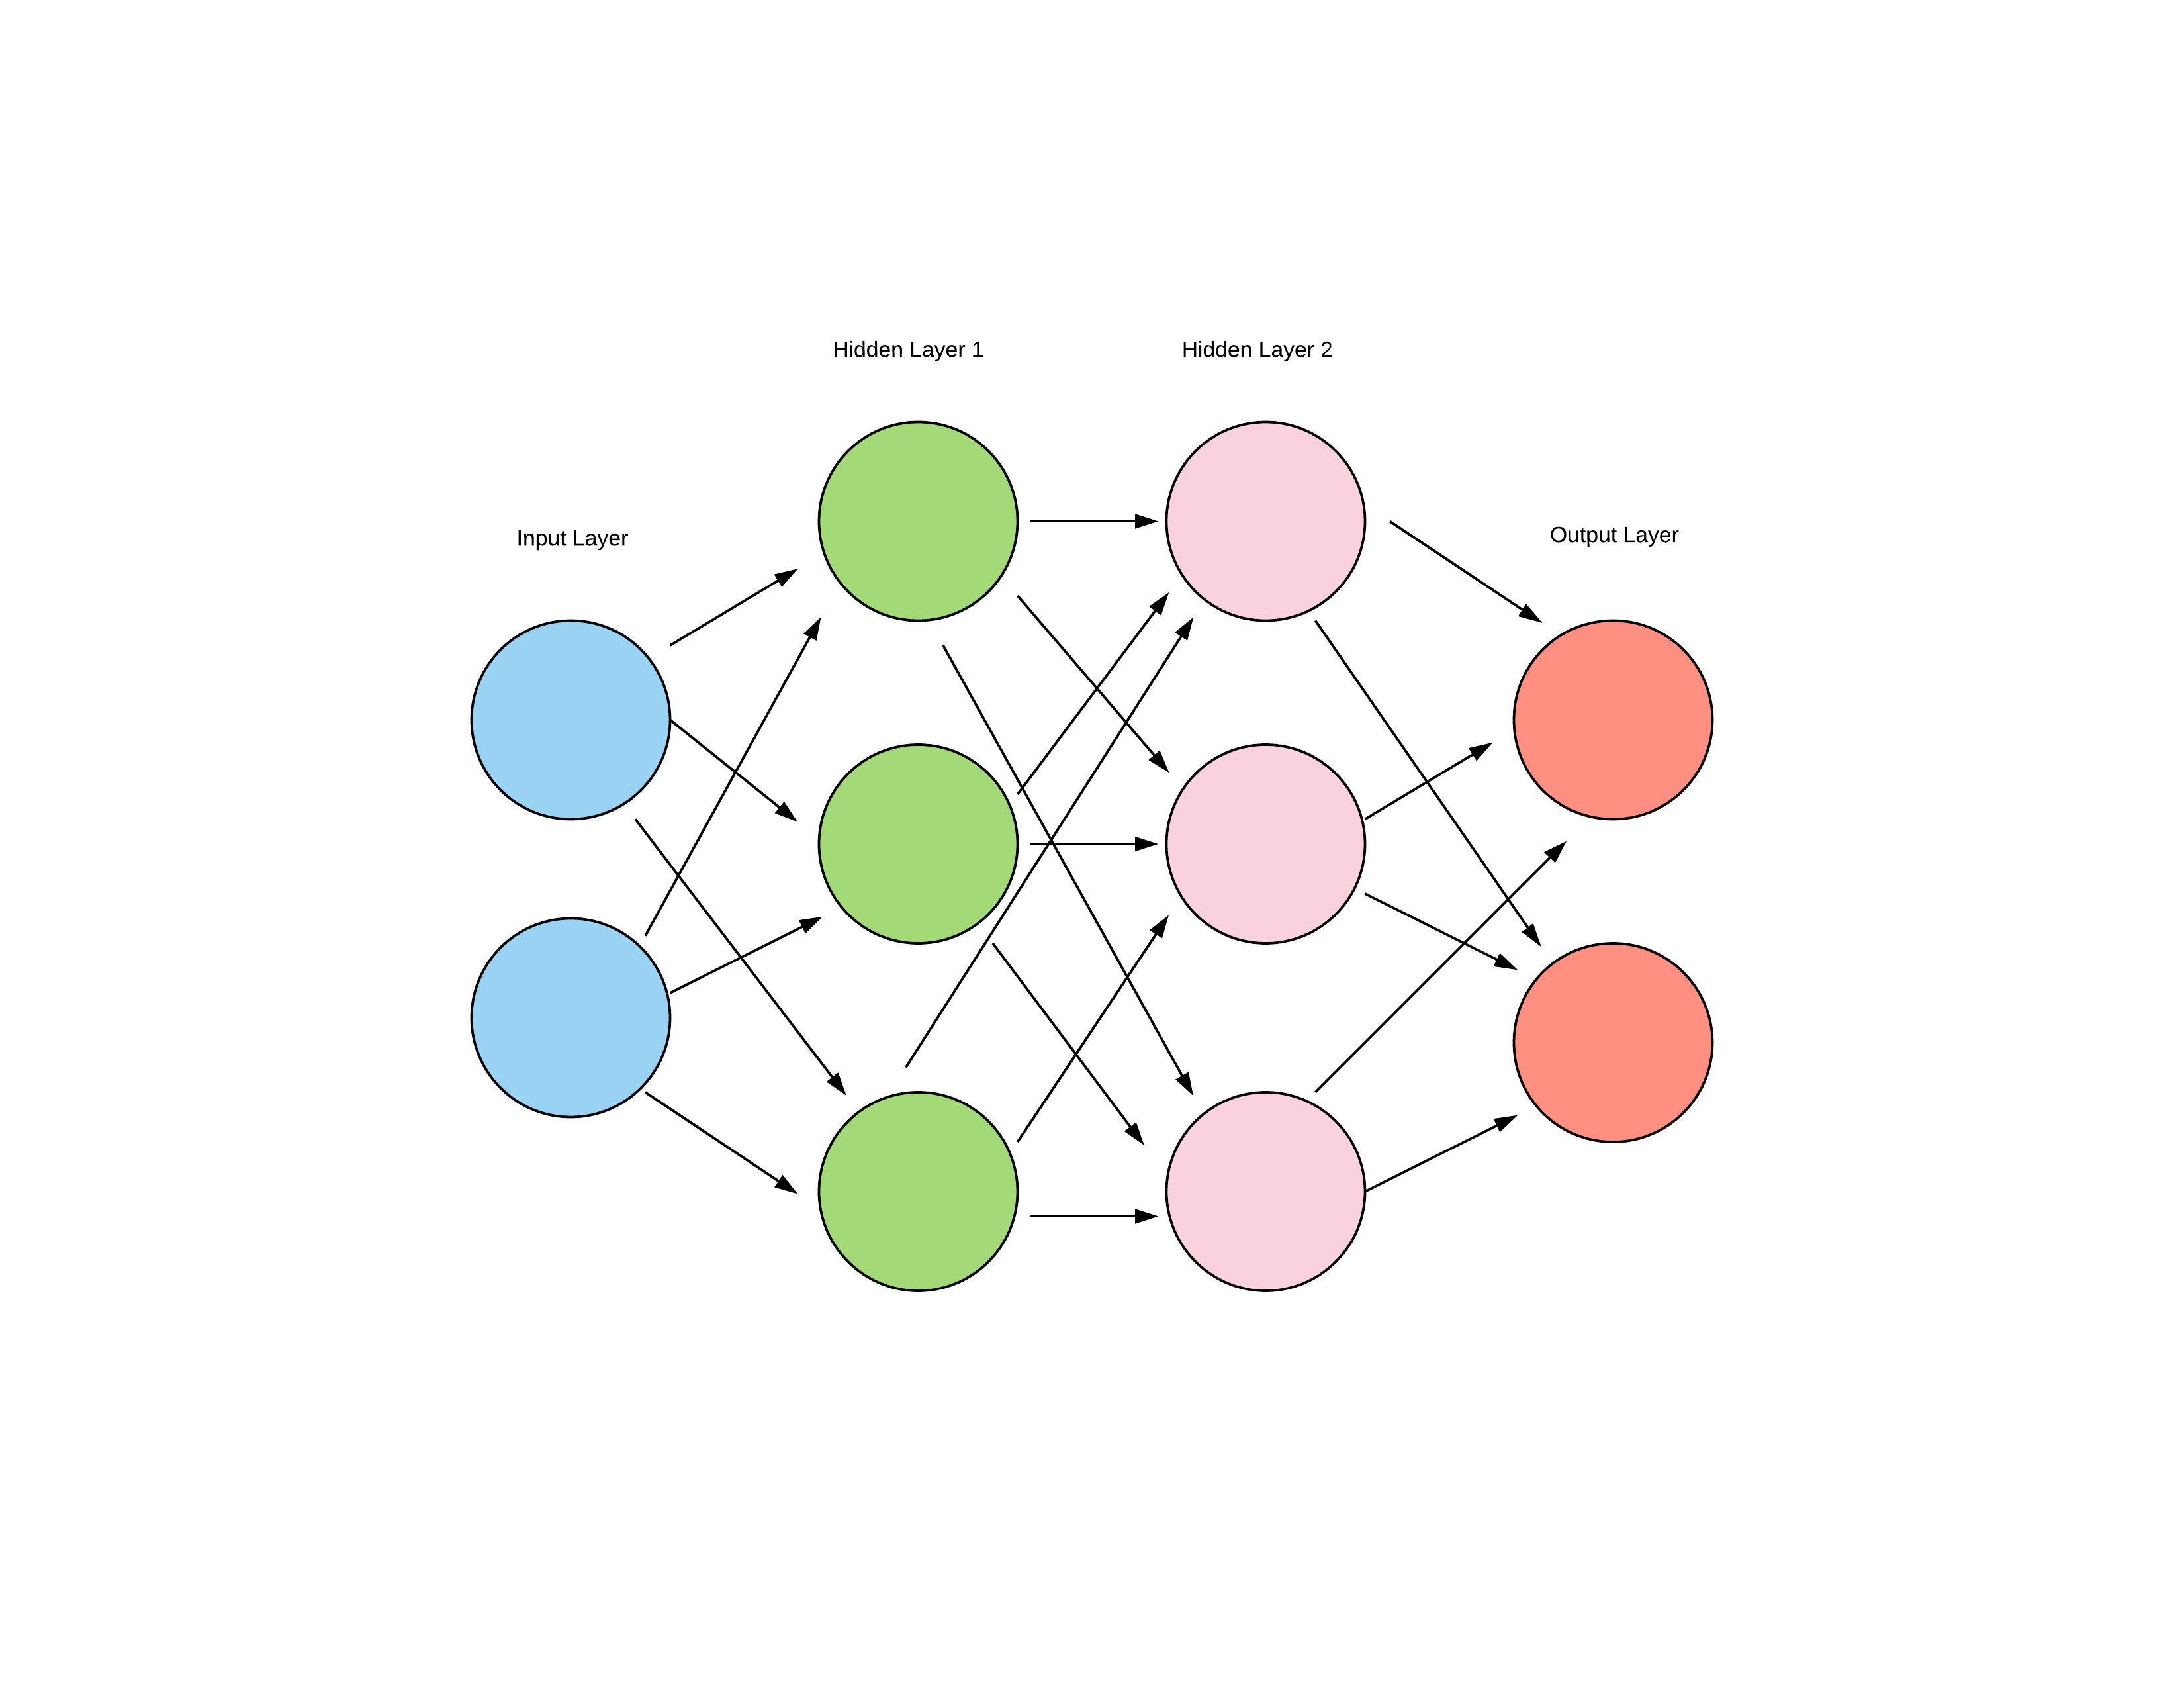
\includegraphics[width=150mm,scale=0.5]{mlp}
    \caption{Multi Layer Perceptron}
    \label{fig:mlp}
\end{figure}

The input layer of a network consists of the data that is fed into the network to be classified. The input layer passes this data to a hidden layer
whose purpose is to transform this data into something that the output layer can
understand. This transformation results in a linearly separable space that can be classified. The output layer normally consists of a class prediction.

MLPs are a class of feed forward ANNs.
These means that the output of each perceptron feeds into an input in the next
layer of the network, example seen in Figure \ref{fig:mlp}.

During training, using backpropagation for each step, the output of every neuron is calculated in each layer and then passed to the next layer. Then the error of the output is calculated, and the network calculates how each neuron in the last hidden layer effected the error. This is continued back through all the layers until the input layer \parencite{handsOnML}. The weights are then altered to try and reduce this error.

There is one large problem with MLP's and as a result CNNs were created. If one is attempting to classify images with a MLP then
each pixel in that image would have to be a separate input. This creates a
massive number of neurons through all the layers and this isn't feasible. CNN's
solve this problem which we will discuss later.



\tocless\subsubsection{Gradient Descent and backpropagation}
Gradient descent is an algorithm used to find the optimal weights to produce the
smallest prediction error. It is used to overcome problems of non-linearly
separable classes. Gradient descent search selects a random weight value and
then modifies it gradually to minimize the error. "At each step, the weight
vector is altered in the direction that produces the steepest descent along the
surface" \parencite{MLANN}. This step is iterated until the lowest value is met.

There is an error function used for the perceptron which finds the lowest error for that neuron, but it can't be used here because, since we have many neurons, there could be an error in multiple neurons.
Gradient descent is mathematically based on the derivative of a function.
The gradient of a function can be calculated by differentiating it.
As the weights are what is being controlled, "they are what we differentiate in respect to" \parencite{MLAlgorithm}.
The negative gradient of this function is followed to find the lowest possible point, hence the name gradient descent \parencite{MLAlgorithm}.

One problem with gradient descent is that if we look at Figure \ref{fig:GD}, we may
never get to the optimal point, point B. This is because we will find point A
without too many problems but when the weights change we will get too high a
slope of error and therefore will never reach point B.

Another variation of gradient descent is Stochastic Gradient Descent (SGD). SGD
is different because it updates "weights incrementally, following the
calculation of the error of each individual example" \parencite{MLANN}. 

\begin{figure}[h]
      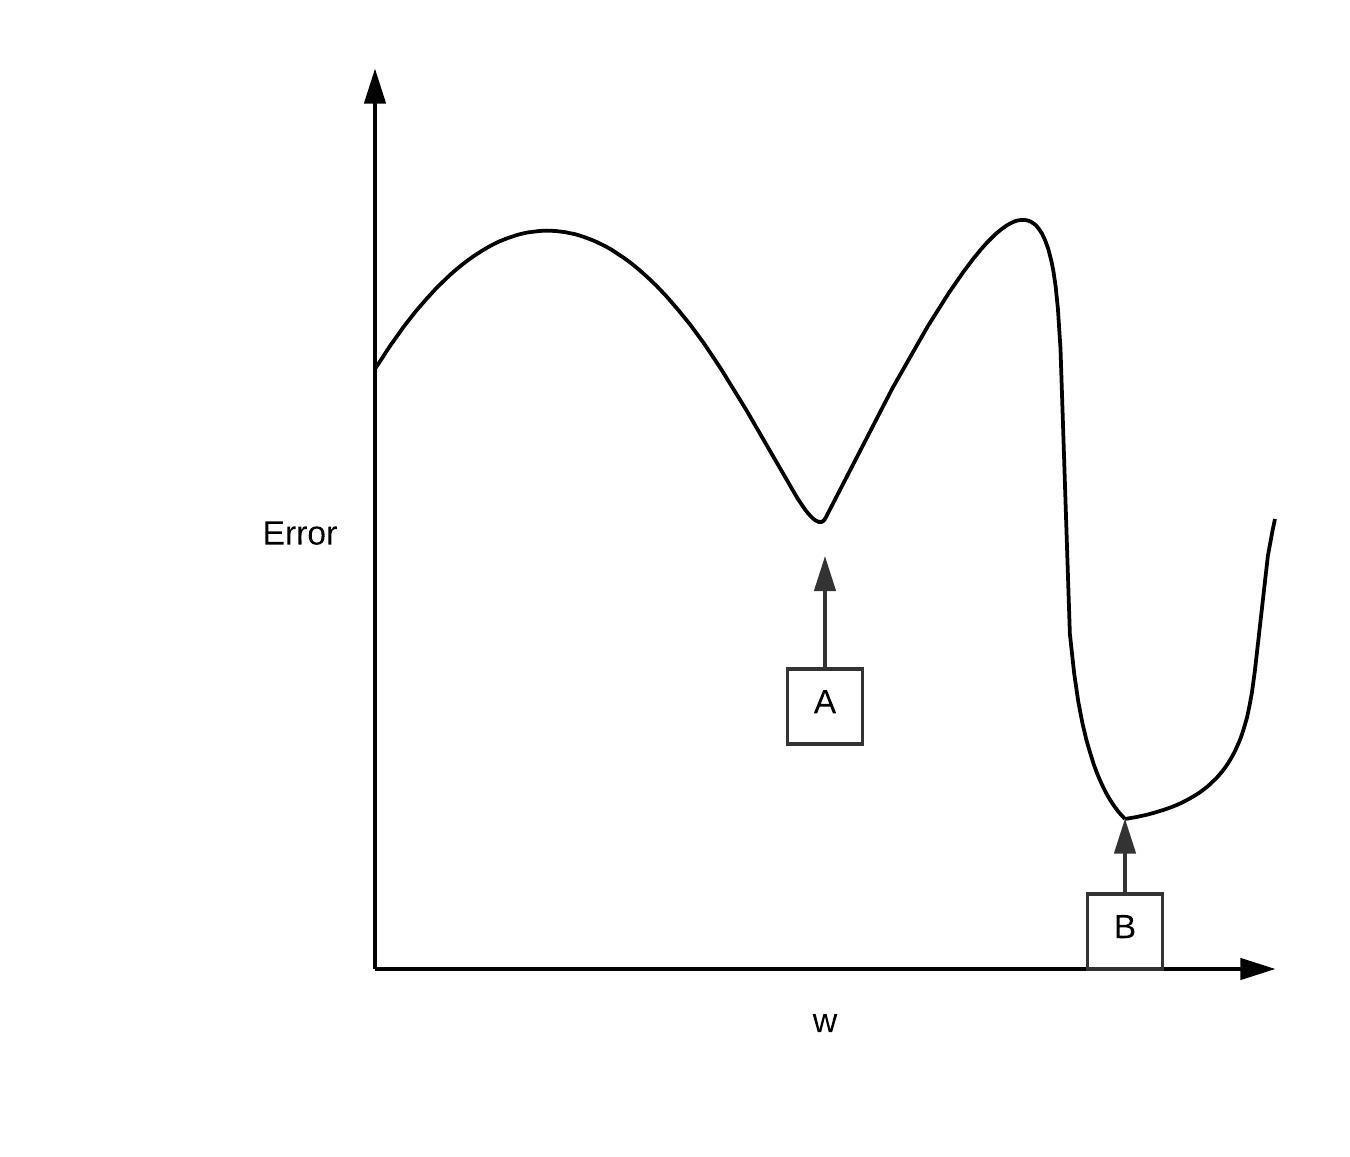
\includegraphics{GradientDescent}
      \caption{Gradient Descent}
      \label{fig:GD}
 \end{figure}

"The Backpropagation algorithm learns the weights of a multilayer network,
given a network with a fixed set of units and interconnections" \parencite{MLANN}.
Backpropagation attempts to minimize the mean squared error between the target
output and the actual output of a network.

Backpropagation works by starting at the output layer of the network and going
back through previous hidden layers, updating weights as it goes i.e. it propagates back through the network, updating the weights to try and reduce the error.

\parencite{MLANN} defined a walkthrough of the backpropagation algorithm.
For every value of Equation \ref{eqn:bp1}, in the training set where x is a vector of inputs and t is a vector of output values to act as a target:
\begin{itemize}
	\item{Run x through the network and output Equation \ref{eqn:bp2}.}
	\item{For each output k, calculate the error by Equation \ref{eqn:bp3}.}
	\item{For every hidden unit, calculate the error by Equation \ref{eqn:bp4}.}
	\item{Update weights by Equation \ref{eqn:bp5} where Equation \ref{eqn:bp5} is true.}
\end{itemize}

\begin{equation}\label{eqn:bp1}
    \vec{x}, \vec{t}
\end{equation}

\begin{equation}\label{eqn:bp2}
    o_{u}
\end{equation}

\begin{equation}\label{eqn:bp3}
    \delta_{k} \leftarrow o_{k}(1 - o_{k})(t_{k} - o_{k}) 
\end{equation}

\begin{equation}\label{eqn:bp4}
    \delta_{h} \leftarrow o_{h}(1 - o_{h}) \sum_{k \in outputs}   w_{kh}\delta_{k}
\end{equation}

\begin{equation}\label{eqn:bp5}
    w_{ji} \leftarrow w_{ji} + \Delta w_{ji}
\end{equation}

\begin{equation}\label{eqn:bp6}
    \Delta w_{ji} = \delta_{j} x_{ji}
\end{equation}


\section{Convolutional Neural Networks Overview}
Convolutional Neural Networks (CNN's) are essentially a Multi Layered Percetron with a
special structure. CNN's have one major difference from a MLP, they have extra
layer of convolution and pooling. The architecture of a convolution network can
be seen in Figure \ref{fig:convNet}.

\begin{figure}
	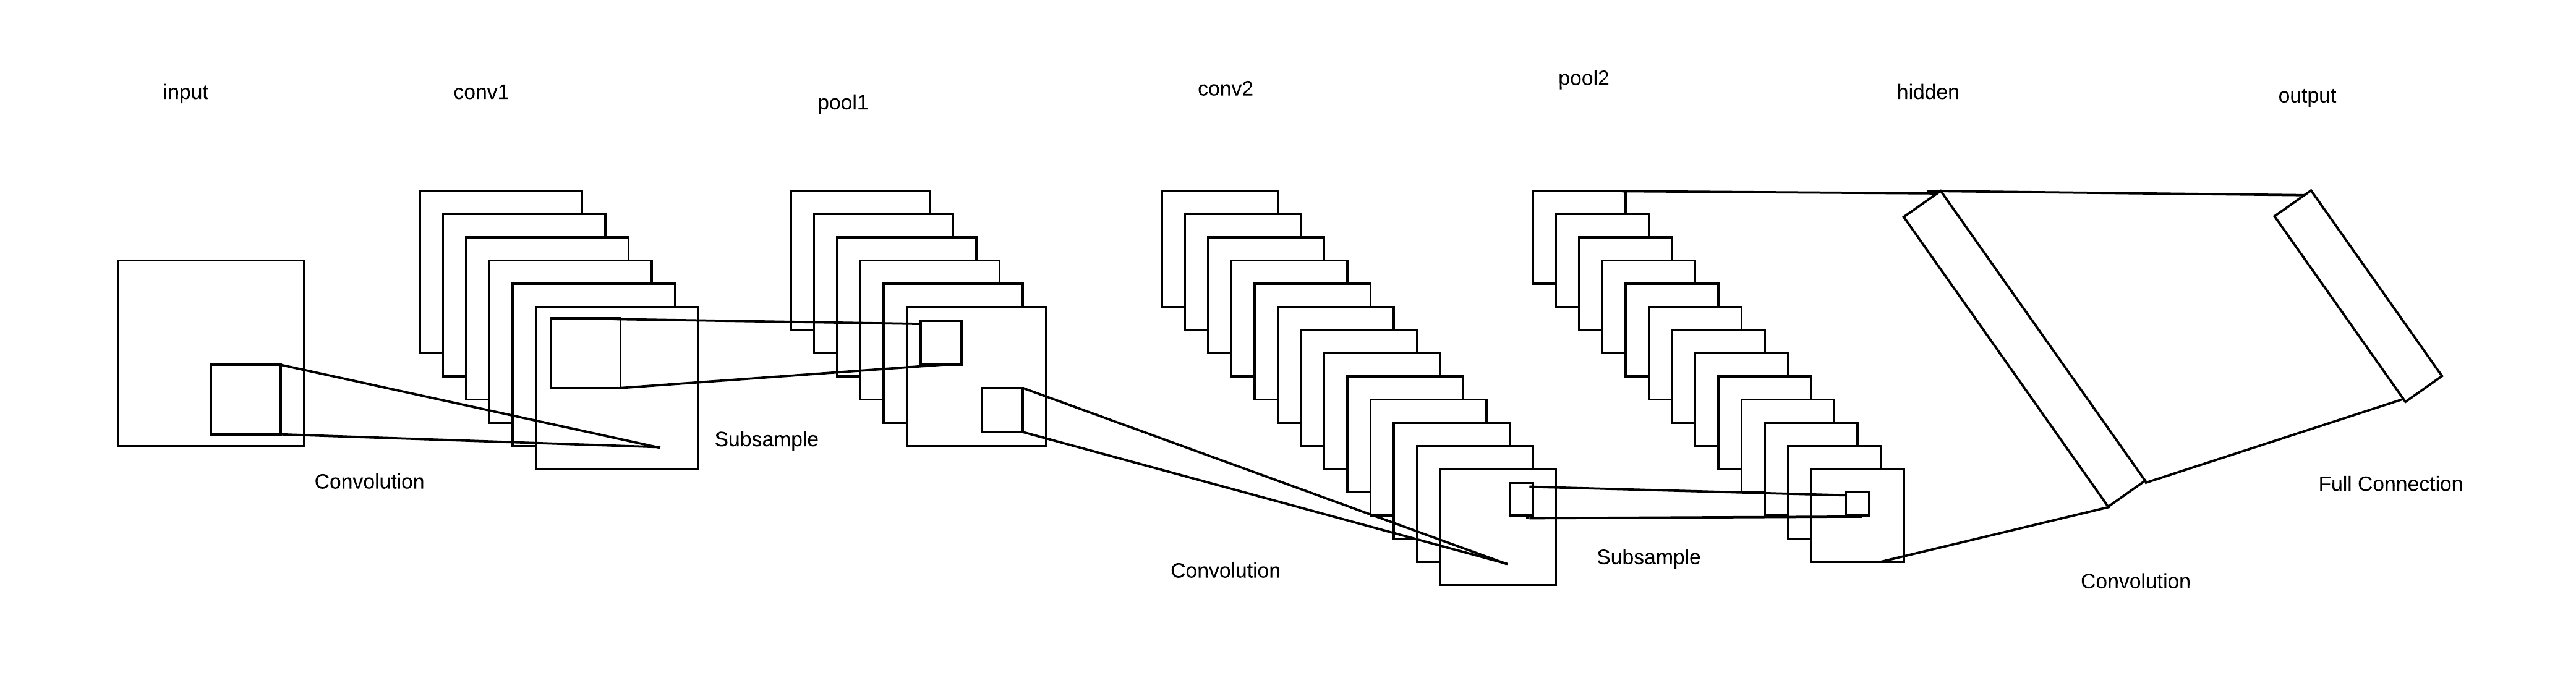
\includegraphics[width=150mm, scale=0.5]{convNet}
	\caption{CNN Architecture}
	\label{fig:convNet}
\end{figure}

Figure \ref{fig:XtoRec} show an image that we want to compare against
Figure \ref{fig:XtoComp}.
For humans, it is quite easy to determine that these images are very similar but
for a computer this task is surprisingly difficult.

So what a CNN does, to combat this problem, is to take a small feature from
Figure \ref{fig:XtoRec} and compare it to a subsection of Figure \ref{fig:XtoComp}.
The CNN multiplies the feature and a section of Figure \ref{fig:XtoComp}, adds
up the results and divides by 9. This then gives a decimal value of how likely
it is that the feature is in the part of the image, as seen in Figure
\ref{fig:convoluted}.
This is called filtering. The Convolutional layer is composed of carrying out
this filtering for every single possible location in Figure \ref{fig:XtoComp}.
\begin{figure}
	\caption{Image filtering}
    \label{fig:filter}
      \begin{subfigure}[b]{0.4\textwidth}
          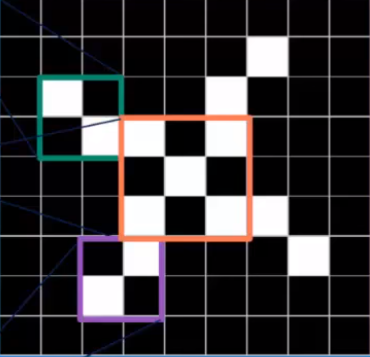
\includegraphics[width=\textwidth]{XtoRec}
          \caption{Image to Classify}
          \label{fig:XtoRec}
      \end{subfigure}
    %
      \begin{subfigure}[b]{0.4\textwidth}
      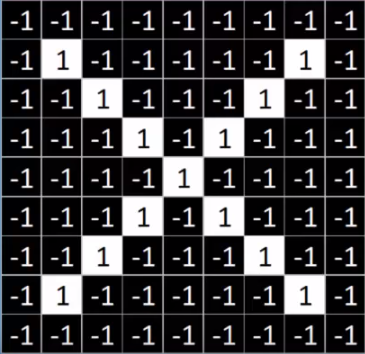
\includegraphics[width=\textwidth]{XtoComp}
      \caption{Image to Compare}
      \label{fig:XtoComp}
      \end{subfigure}
\end{figure}

\begin{figure}
    \caption{Image Convolution}  
    \begin{subfigure}[b]{0.4\textwidth}
          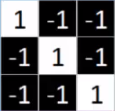
\includegraphics[width=\textwidth]{ImageFeature}
          \caption{Image Feature to Search}
          \label{fig:feature}
      \end{subfigure}
     %
      \begin{subfigure}[b]{0.4\textwidth}
           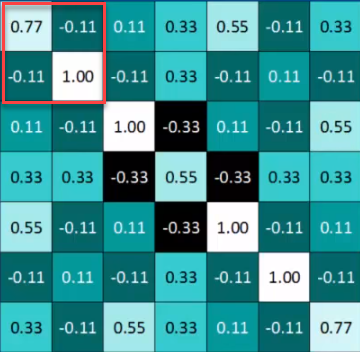
\includegraphics[width=\textwidth]{ConvImage}x
           \caption{Convoluted Image}
           \label{fig:convoluted}
      \end{subfigure}
\end{figure}
\begin{figure}
    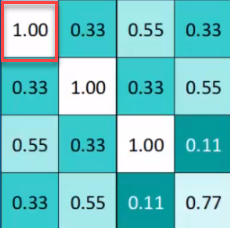
\includegraphics[width=50mm,scale=0.5]{PooledImage}
    \caption{Pooled Image}
    \label{fig:pooled}
\end{figure}
Next is the Pooling Layer, what this layer does, is it takes the convoluted
layer output, you can use Figure \ref{fig:convoluted} as reference, and from a
user defined size ie. 2x2, gets either the highest decimal value (Max pooling)
or the average value (Mean pooling) and records that as the new value for the
section. This is then applied to the entire image. As we can see in Figure
\ref{fig:pooled} we know have a much smaller image stack in which to classify,
thus making the computation easier.

In between the Convolution and Pooling layer, there is sometimes a Normalization
layer. This Normalization layer creates Rectified Linear Units (RLU's). In other
words, if we take Figure \ref{fig:convoluted}, it changes all minus values to
zero.

There are some problems with CNN's however. One of the main problems is that you
need a very large dataset in order to produce am accurate model and the training
can be very time consuming without a GPU.

\section{Convolution Neural Networks Extended}

\subsection*{Fully Convolutional Networks}
A Fully Convolutional Network is one that does not have a fully connected layer
and in a fully connected layers place is another convolution layer.

\section{Support Vector Machine}
A Support Vector Machine (SVM) is a machine learning algorithm that has been
very popular before the use of a CNN was mainstream.
Many of the texts that will be analysed later use SVMs for their classification.

A SVM works by creating an n-dimensional space, with n as the number of
inputs you have \parencite{svm}. The SVM algorithm finds the hyperplane that splits this space.
This hyperplane can then be used for classification. 
An SVM casts the problem to a higher dimensional space and this can solve a problem when the classes are not linearly separable.
This can be seen in Figure \ref{fig:svm}, where on the left there is no clear way to separate the classes but once the problem is cast to another dimensional, the separation is clear.

\begin{figure}[h]
    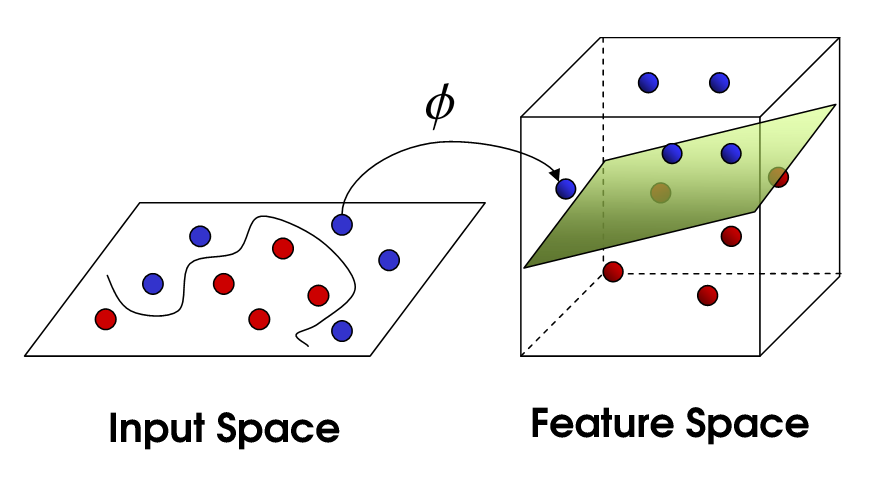
\includegraphics[scale=0.35]{svm}
    \caption{Support Vector Machine Applicability sourced from https://stackoverflow.com/questions/9480605/what-is-the-relation-between-the-number-of-support-vectors-and-training-data-and}
    \label{fig:svm}
\end{figure}

There are benefits and liabilities to using a SVM.
They can be very accurate and can work efficiently with small datasets but unfortunately it can take a large amount of time to train. 

\section{Evaluating the Output}
There are various different metrics that can be used for evaluating the output
of a classifier or segmentation algorithm, many of which we have seen in previous
sections. I was analyse a few of these evaluations of results so that I can use
them as a reference to apply to my own experiments. I will also look into some
problems associated with evaluating models.

\subsection{Research into Diagnosing Errors in Object Detectors}
There has been some research into the question of how to evaluate object
detectors, one of which I will discuss in detail \textcite{diagnosingErrors}.
This paper in question "analyzes the influences of object characteristics on
detection performance and the frequency and impact of different types of false
positives" \textcite{diagnosingErrors}. They found that there were many effects
that had influence on detectors as follows:
\begin{itemize}
    \item{occlusion}
    \item{size}
    \item{aspect ratio}
    \item{visibility of parts}
    \item{viewpoint}
    \item{localization error}
    \item{confusion with semantically similar objects}
    \item{confusion with other labeled objects}
    \item{confusion with background}
\end{itemize}

The research team goes on to analyse false positives in object detectors.
Localization errors were a large factor. This is were bounding boxes overlap to
other objects in the image. Confusion with similar objects had a large influence
on false positives also by which, for example, a dog detector had a high score
for a cat \textcite{diagnosingErrors}. Confusion with dissimilar objects and
confusion with background are the categories of the rest of the false positives
they measured.

In conclusion the team would that "Most false positives are due to misaligned
detection windows or confusion with similar objects"
\textcite{diagnosingErrors}. They had some recommendations towards improves
detectors as follows:
\begin{itemize}
	\item{Smaller objects are less likely to be detected}
	\item{Localization could be improved}
	\item{Reduce confusion with similar categories}
	\item{Robustness to object variation}
	\item{More detailed analysis}
\subsection{Detection Average Precision}
See \ref{fig:dap}.
\begin{figure}
	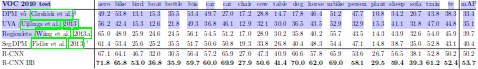
\includegraphics[width=150mm,scale=0.5]{DAP}
	\caption{Detection Average Precision \textcite{donahue}}
    \label{fig:dap}
\end{figure}

\subsection{Mean Average Precision}
See \ref{fig:MAP}.
		\begin{figure}
			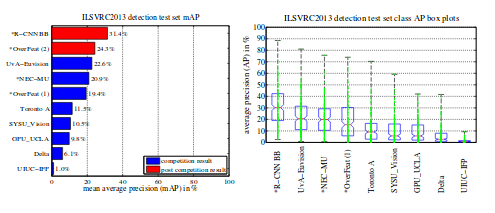
\includegraphics[width=150mm,scale=0.5]{MAP}
			\caption{Mean Average Precision \textcite{donahue}}
			\label{fig:MAP}
		\end{figure}
		
\subsection{Distribution of top-ranked false positives}
See \ref{fig:DFP}.
		\begin{figure}
			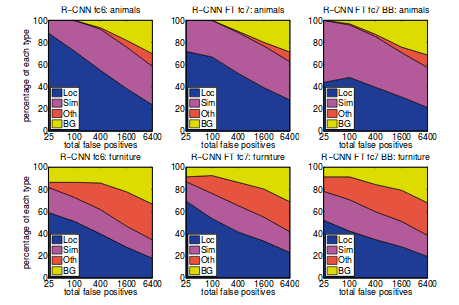
\includegraphics[width=150mm,scale=0.5]{DFP}
			\caption{Distribution of top-ranked false positives \textcite{donahue}}
			\label{fig:DFP}
		\end{figure}
		

\subsection{Segmentation Mean Accuracy}
See \ref{fig:SMP}.
		\begin{figure}
			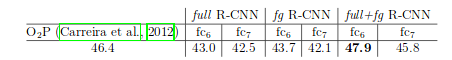
\includegraphics[width=150mm,scale=0.5]{SMP}
			\caption{Segmentation Mean Accuracy \textcite{donahue}}
			\label{fig:SMP}
		\end{figure}
		

\subsection{Per-category segmentation accuracy}
See \ref{fig:PCATSA}.
		\begin{figure}
			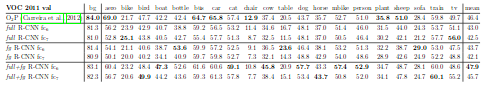
\includegraphics[width=150mm,scale=0.5]{PCATSA}
			\caption{Per-category segmentation accuracy \textcite{donahue}}
			\label{fig:PCATSA}
		\end{figure}
		

\subsection{Per-class segmentation accuracy}
\See \ref{fig:PCLASSA}.
		\begin{figure}
			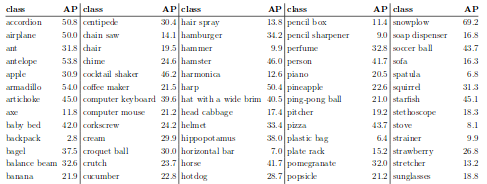
\includegraphics[width=150mm,scale=0.5]{PCLASSSA}
			\caption{Per-class segmentation accuracy \textcite{donahue}}
			\label{fig:PCLASSA}
		\end{figure}
		



\section{Dietary Assessment using Computer Vision}
\subsection{Convolution Neural Networks}
Many researchers have used convolutional neural networks for image
classification with various network architectures and many have used a food image dataset.
Some of these papers will be looked at below.
A summary of their results can be seen in Table \ref{cnn_summary}.

\parencite{deepLearning} focused on a deep learning approach to food image recognition based
their neural network architecture on Inception-ResNet and Inception V3.
Deep learning is a term usually given to algorithms based on neural networks.
They also used the Food-101 dataset. For this system, Google's
Tensorflow was used for image preprocessing. Preprocessing was needed as the
environmental background is different in many food images. Because of these
"Grey World method and Histogram equalization" \parencite{deepLearning} were
used.
Amazon Web Services (AWS) Graphics Processing Units (GPU) instances were used for training.
AWS instances are cloud servers.
The results on completion were quite impressive with a Top-1 Accuracy of 72.55\% and a Top-5 Accuracy of 91.31\%.

Another research team in Japan, \parencite{yanaiFood} researched this topic. This was built off previous research they had carried out in the field \parencite{kawano2014food}.
They were aware of how
difficult the problem was and therefore employed many techniques to solve the
problem such as "pre-training with the large-scale ImageNet data, fine-tuning
and activation features extracted from the pre-trained DCNN". 
In conclusion, they found that the "fine-tuned DCNN which was pre-trained
with 2000 categories" from ImageNet was the best method. A
DCNN is a Deep Convolution Neural Network. 
A network can become a DCNN when the number of hidden layers is larger than three.
While many of the CNNs discussed have been DCNN, most are just labeled as CNNs.
The achieved results of 78.77\% for Top-1 Accuracy in the UECFOOD100 dataset.


\parencite{kagayaFood} also employed the use of convolutional neural networks for
image detection. They used a CNN for the "tasks of food detection and recognition
through parameter optimization".
They found that a CNN is much better suited to the task than a Support Vector
Machine (SVM). They achieved an overall classification accuracy of 93.8\%
against their baseline accuracy of 89.7\%. This accuracy
was calculated using a dataset that they created specifically for this task.
When they had completed the task they analysed the trained convolutional kernels
and came to an interesting conclusion. They found that "color features are
essential to food image recognition".


The last paper that will be analysed, \parencite{deepFood}, oriented around using a Convolutional Neural
Network for food image recognition, focuses on developing a dietary assessment
application for use on a smart phone. They used the UEC-256 and Food-101 dataset
for their experiments and achieved impressive results.
They used a Convolutional Neural Network but "with a few major optimizations,
such as optimized model and an optimized convolution technique". 
They used the Inception module for their CNN. After the
inception module was complete, they made the GoogleNet architecture by combining modules. In
total, the network had 22 layers.
They achieved the results shown in Table \ref{resultsDeepFood}.

\begin{table}[h]
	\centering
	\caption{DeepFood Results}
	\label{resultsDeepFood}
	\begin{tabular}{lll}
		& Top-1  & Top-5  \\
		UEC-256                   & 54.7\% & 81.5\% \\
		UEC-100                   & 76.3\% & 94.6\% \\
		Food-101                  & 77.4\% & 93.7\% \\
		UEC-256 With Bounding Box & 63.8\% & 87.2\% \\
		  UEC-100 With Bounding Box & 77.2\% & 94.8\%
	\end{tabular}
\end{table}

\parencite{nutrinet} developed a new neural architecture specifically for detecting food and drink images using deep convolutional neural networks called NutriNet.
The trained network was to be used to aid patients with Parkinson's disease in monitoring their diet.
NutriNet was created based off of the AlexNet architecture.
The dataset used for this study consisted of approximately 500 images for each of over 500 classes.
Through this dataset a Top-1 accuracy of 86.72\& and a Top-5 accuracy of 94.47\% was recorded.
A smart phone application was used for real world testing which brought a Top-5 accuracy of 55\%.
The application also saved these real world images from the smart phone to increase their dataset size.
In conclusion, the team found that there were modifications that could be made to the NutriNet architecture as real world images didn't perform incredibly well due to occlusion and background noise in the images.
The detection and recognition steps were separated in this architecture.
The team also acknowledges that joining these steps into a single DCNN may be successful and should be explored.

\begin{table}[h]
	\centering
	\caption{Summary of results in CNN based methods}
	\label{cnn_summary}
	\begin{tabular}{lll}
		Title                                & Dataset     & Top-1 Accuracy \\
		\parencite{deepLearning} 			 & Food 101    & 72.55\%  \\
		\parencite{yanaiFood}               	 & UECFood101  & 78.77\%  \\
		\parencite{kagayaFood}       		 & Own dataset & 93.80\%   \\
		\parencite{deepFood}                  & Food 101    & 77.40\%  	\\
		\parencite{nutrinet}                  & Own dataset & 86.72\%
	\end{tabular}
\end{table}



\subsection{Support Vector Machines}
While Convolutional Neural Networks have proven very successful in recent years, there are many other methods of food image identification and classification that have been employed by food image recognition researchers, such as SVMs.
A summary of the results of these methods can be seen in Table \ref{other_dietary_summary}.

In a study conducted by \parencite{kernelLearning}, a practical use for food image recognition in the form of a mobile phone application was proposed.
In order to classify the images, multiple kernel learning(MKL) was used.
MKL is similar to a SVM expect that instead of a single kernel during training, MKL " treats with a combined kernel which is a weighted linear combination of several single kernels" \parencite{kernelLearning}.
The idea behind this is that different food types are distinguishable by different factors and using this method, the best of these factors can be used for classification of that food type.
In the experiments carried out, three different factors were used for learning:
\begin{itemize}
	\item{Colour Histograms}
	\item{Gabor Texture Features}
	\item{Bag-of-Features using Scale Invariant Feature Transformation (SIFT)}
\end{itemize}

According to \parencite{sift}, "SIFT features are formed by computing the gradient at each pixel" in a window and then using the correct level of the Gaussian filters where the window was detected.
50 different classifiers were created in a SVM using MKL with " one category as a positive set and other 49 categories as a negative set" \parencite{kernelLearning}.
For each of these categories, a web scrape was carried out and then the best 100 images for each scrape was manually selected. Five-fold cross validation was utilised in the paper.

MKL proceeded to yield results of 61.34\% on the 50 food types and a Top-3 accuracy of 80.05\%.
The prototype mobile phone application resulted in a 37.55\% user accuracy.
While the Top 1 and Top 5 accuracies for this model show promising results, the user accuracy is very poor.
This would suggest that the classifier does not work well with real life images and is possibly overfitting to the training and testing dataset.
MKL classifiers may not be promising for generalisation.

Another quite successful study was carried out using a SVM.
\parencite{novelSVM} had established that both colour and texture are very important, but they also decided that shape and size are vital features to analyse.
The proposed system has two main parts, segmentation followed by classification.
To create a 'robust' system, a 'Robust Handling of Different Lighting Conditions' module is added to the system \parencite{novelSVM}.
This is so that various lighting conditions don't cause colour data to be distorted. 

Since this paper calls for calorie estimation, the first step of the system calculates the size of the food portion. In order to do this, a coin or the users thumb is included in the image taken so that the pixel count of the thumb and the food can be compared to estimate the size. Following this the image is segmented into various portions. The following step classifies each segment of the image by extracting colour, texture and shape features and inputting these into a SVM.

12 different food types were trained for this SVM with an average classification accuracy of 92.6\%.
\parencite{novelSVM} came to the conclusion that it would be difficult to use their algorithm with real data and no evidence of real-world testing was recorded.
This is unfortunate as it is difficult to get an idea of the success of the system.
Unfortunately, only 12 food types were trained and no evidence is given of how the classifier scales to more classes.

Another study that employed both a SVM and an emphasis on colour, texture and shape features, was carried out by \parencite{pouladzadeh2014measuring}.
Size was also a factor in the calorie measurement module of the system. It was found that using all four of these features increases the overall accuracy.

In order to segment the image successfully, Gabor filters were applied to separate texture features while colour was also utilised. For each segment established, size, shape, colour and texture features were extracted and using a SVM, a classification was made. The SVM used the radial basis function kernel.
Calorie estimation was also a large part of this paper, and the users thumb was taken with the food to calculate food size.

In the prototype application, once the classification had been made, the user can confirm or change the prediction. Another feature of the application was in regards to " Partially Eaten Food" \parencite{pouladzadeh2014measuring}. This was accomplished by taking a picture before and after consumption and as a result only calculated the size of the food eaten and therefore more accurate calorie counts can be produced.

15 food types were trained using the SVM with 3,000 images. The accuracy for the classifier averaged at 90.41\% using 10-fold cross-validation.
There was also a calorie count accuracy of 86\%. The best classification results were on single foods followed by non-mixed and finally mixed foods produced the worst results.

Even though \parencite{pouladzadeh2014measuring} segmented the image before classification, they still had poor results on mixed foods.
The low number of classes the classifier was trained on makes it difficult to see how effective the classifier is.
It would also be beneficial to know how long classification took on a new image as the classifier used features of colour, texture, size and shape which would be quite time consuming.

\parencite{zhu2011segmentation} had a strong focus on the segmentation aspect of a dietary assessment system.
The segmentation of the food images was achieved " using Normalized Cuts based on intensity and colour" \parencite{zhu2011segmentation}.
Normalized Cuts is a graph-based segmentation method.
To aid the segmentation aspect of this study, a common background colour was introduced to the images.
Segmentation refinement was also an important module in the experiment.
This is the process by which neighbouring segments with  the same classification label are merged together.
This also helps calculate a more accurate size estimation.
The classification of the segmented image was processed by using a SVM calculating colour and texture features.
Gabor filters were used for the texture feature extraction.

In the experimental results for this study, it was found that segmentation was not always successful " when the region of interest is camouflaged by making its boundary faint" \parencite{zhu2011segmentation}. In their case, it was a can of coke that wasn't segmented correctly.
The classification accuracy was of 56.2\% and 95.5\% with ground truth segmentation data.
19 classes of food were used in this study with approximately 60 images per class.
Very little information was given in this paper on the classifier used.
The low classification results do not yield promising results for this method.

% % \tocless\subsubsection{Promising Approaches of Computer-supported Dietary Assessment and Management: 
% % Current Research Status and Available Applications}
% % \parencite{arens2015promising}

% \tocless\subsubsection{Novel Technologies for Assessing Dietary Intake: Evaluating the
% Usability of a Mobile Telephone Food Record Among Adults and Adolescents}
% \parencite{novelTech}

There was a study carried out on food identification through a smart phone application by \parencite{chen2012automatic}.
This study resulted in an application that allows a user to send an image of their food to a server which can give them an automatic response in 12 seconds.
This back-end service can have 34 threads working concurrently as stated at the time the paper was published.

A SVM is used to classify the image across 50 categories trained on around 100 images each.
The SVM uses SIFT and Local Binary pattern feature extractors.
A separate SVM was trained for each of these extractors and was merged together using a " Multi-class AdaBoost algorithm" \parencite{chen2012automatic}.

The study produced a top-1 accuracy  of 68.3\%. Accuracy of 80.6\%, 84.8\% and 90.9\% were recorded using top-2, top-3 and top-5 accuracy respectively.
Unfortunately, real-world image classifcation results were not recorded from the smartphone applications.
Due to this, it is difficult to measure the efficacy of the classifier, even more so because they only had 50 classes.  

% % \tocless\subsubsection{An Overview of the Technology Assisted Dietary Assessment Project at Purdue University}
% % \parencite{khanna2010overview}

\parencite{villalobos2012image} researched the question of using a computer vision approach to this topic. They focus mostly on the segmentation and region of interest calculation of the system in their study.

The system in question requires two images of the food, one from above and one from the side. This helps with size estimation. The users thumb is required to be in the image for accurate size estimation. The application also requires an image after consumption as to not calculate calories for uneaten food.
The system segments the image and then extracts colour, size and shape information from each segment. This data is then used by a SVM for classification along with a nutritional database for calorie information. 
Multiple segmentation methods were tested such as:
\begin{itemize}
	\item{Semi-automatic contour definition}
	\item{Watershed transformation}
	\item{Colour rasterization}
	\item{Edge accentication}
\end{itemize}
The first two were dismissed due to poor results but the second two were used in conjunction for the segmentation aspect of the system.
\parencite{villalobos2012image} did not provide extension information on the classifier used in this study and would be therfore very difficult to replicate.
However, impressive segmentation results were obtained.

An application called "Snap-n-Eat" was proposed by \parencite{snap}.
When an image is taken using this application, the system finds saliency regions to remove the background of the image.
If the image has multiple food types present, hierarchical segmentation takes place before proceeding to a SVM. Similar segments are merged together.
These are found by using colour, texture and size.

SIFT and Histogram of Oriented Gradients (HOG) feature extractors are used on the image and these features are used by the SVM for classification.
The SVM is trained using Scholastic Gradient Descent.
\parencite{snap} also uses a Bog of Visual Words model along with k-means clustering.
An accuracy of 85\% on 15 classes was recorded using this method.

\begin{table}[]
\centering
\caption{Summary of accuracy in dietary assessment methods}
\label{other_dietary_summary}
\begin{tabular}{|p{9cm}|l|l|}
\hline
\textbf{Title}                                                         & \textbf{Classes} & \textbf{Accuracy}   \\ \hline
Food Image Recognition with Multiple Kernel Learning          & 50             & 61.3\%    \\ \hline
A Novel SVM Based Food Recognition Method                     & 12             & 92.6\%     \\ \hline
Measuring Calorie and Nutrition from Food Image               & 15             & 90.4\%    \\ \hline
Segmentation Assisted Food Classification                     & 19            & 56.2\%     \\ \hline
Large Scale Leaning for Food Image Classification             & 11             & 78.0\%       \\ \hline
Toward Dietary Assessment via Mobile Phone Video Camera       & 20             & 92.0\% \\ \hline
Automatic Chinese Food Identification and Quantity Estimation & 50             & 68.3\%     \\ \hline
Food Recognition and Nutrition Estimation on a Smartphone      & 15             & 85.0\% \\ \hline      
\end{tabular}
\end{table}

\subsection{Other Methods}
Methods outside of CNNs and SVMs are outlined below.
A summary of the results can be seen in Table \ref{other_dietary_summary} along with SVM method results.

\subsubsection*{Large Scale Learning for Food Image Classification}
\parencite{LSL_2015} proposed a food image recognition system using a Bag of Features model.
This study used over 5000 images separated into 11 classes.

A clustering algorithm was employed on this study before classification.
For the classification step, experiments were carried out using different methods:
\begin{itemize}
	\item{SVM}
	\item{ANN}
	\item{Random Forests}
\end{itemize}

The final accuracy of the system was 78\% \parencite{LSL_2015}.

% % \subsubsection*{Promising Approaches of Computer-supported Dietary Assessment and Management: 
% % Current Research Status and Available Applications}
% % \parencite{arens2015promising}

\subsubsection*{A Personal Assistive System for Nutrient Intake Monitoring}
Similar to other approaches seen thus far, \parencite{personalAssistive} employs the use of the users thumb in the image for size estimation.

Once a photo has been taken by the user with their thumb present, the system segments the food on the plate using shape, colour and texture detectors.
The system then classifies the food type based on these features.

In this paper, it was decided to allow the users to change the prediction by the system.
The thumb of each user is calibrated upon first use of the application so that size estimation can be as accurate a possible \parencite{personalAssistive}.

\subsubsection*{Toward Dietary Assessment via Mobile Phone Video Camera}
Another study into using computer vision for dietary assessment was carried out by \parencite{chen2010toward}. They had a unique medium for the topic by using a video of the dishes in question and extracting frames from these videos to get the food from different angles.

\parencite{chen2010toward} then formed a region of interest in the image, where there were the most food items and extracted colour and image features.
These image features were extracted using Maximally Stable Extremal Regions (MSER), Speeded Up Robust Features (SURF) and Star detector.

This research team also uses k-means clustering to build a bag-of-words model \parencite{chen2010toward}.

The system had results as seen below across 20 categories using five images out of each video taken of the food:
\begin{itemize}
	\item{MSER - 95\%}
	\item{SURF - 90\%}
	\item{STAR - 90\%}
\end{itemize}

% \subsubsection*{Novel Technologies for Assessing Dietary Intake: Evaluating the
% Usability of a Mobile Telephone Food Record Among Adults and Adolescents}
% \parencite{novelTech}


% % \subsubsection*{An Overview of the Technology Assisted Dietary Assessment Project at Purdue University}
% % \parencite{khanna2010overview}

\subsubsection*{Merging dietary assessment with the adolescent lifestyle}
\parencite{schap2014merging} proposed a system used by smart phones which sends an image of a users food to a back end system for computation.

Once this has been completed, the image is segmented, features are extracted from each segment and these segments are classified.
Colour and texture features are used for classification.
The user has the ability to confirm or amend predictions of the food type.

Size estimation is also an important aspect of this system.
In contrast to previous studies, \parencite{snap} uses food type shape and then those shape's geometric properties to estimate size.

This study produced results of 94\% out of 32 test cases.










\section{Object Detection Using CNNs}
Due to the issues with composite images (images with multiple items) in food image recognition, an object detection approach may prove to be successful.
If the objects (different food items) in an image could be classified seperately then the overall effiency of a nutrional assessment system, aided by deep learning, could be improved.
Ross Girshik and other contributors had some very positive results in the area
of object detection using region based convolutional neural networks. There were
four iterations of papers based on this work by Ross and groups in UC Berkley,
Microsoft and Facebook. A PHD student at the time of Ross's first paper also
completed his dissertation on the subject. These papers, their
results (Table \ref{rcnnResults}) and the changes made through each iteration will be analysed thoroughly in the proceeding sections.

In the first paper written by Ross Girshik, while researching at UC Berkeley,
focused on two main insights. These were that " one can apply high-capacity convolutional neural networks (CNNs) to bottom-up region proposals in order to localize and segment objects" and that
"when training data is scarce, supervised pre-training for n auxiliary task,
followed by domain-specific fine-tuning, yields a significant performance boost"
\parencite{rcnn}.

The system that they developed followed these steps:
\begin{itemize}
    \item{Take image as input}
    \item{Extract approximately 2000 region proposals from the image}
    \item{Compute fixed length vectors of features for the regions using a convolutional
        neural network}
    \item{Use a Support Vector Machine (SVM) to classify these regions}
    \item{Bounding box regression for final region proposals}
\end{itemize}

This system utilised selective search to gather these region proposals, but they
mention that a sliding-window detector is also an option. Ross Girshik and his
team used the open source Caffe CNN library for this system. The system is quite
efficient and scalable. It is scalable because of the fixed length vector of
features which will remain constant regardless of inputs and additional outputs.
The team evaluated their results on a few metrics and test sets as seen in Table
\ref{rcnnResults}. Explanation of the datasets used can be seen in Table \ref{datasets}.

Ross Girshik's next iteration of work on region based convolution neural
networks took place in Microsoft Research. This paper was titled "Fast R-CNN" as
its aim was to decrease training and testing time "while also increasing
detection accuracy" \parencite{fastRcnn}.

This paper analyses why RCNN \parencite{rcnn} was slow and therefore how it could be improved.
RCNN was classified to be slow because of three main factors:
\begin{itemize}
	\item{There are multiple stages to training as both a CNN and a SVM need to
		be trained.}
	\item{In training of the SVM, each region proposal must be written to disk
		and is therefore expensive.}
	\item{Object detection takes 47 seconds per image}
\end{itemize}

Due to these problems with RCNN, a new algorithm, titled Fast RCNN was proposed.
The architecture is as follows. An image is taken as input along with a
proposal for regions. The image is pushed through convolutional and pooling
layers (using max pooling). A fixed-length vector of features is then extracted
from each region proposal. These vectors are inputted to fully connected
layers for bounding box location prediction.
At detection time, a pass through of the net is all that is needed so this
runtime is significantly less than RCNN.

Due to the success of RCNN and Fast RCNN, Faster RCNN was introduced to combat
the problem of region proposal computation \parencite{fasterRcnn}.
The architecture for this system comprises of two modules. These consist of a
convolutional neural network for region proposals (RPN) which the feeds into a Fast
RCNN detector. These combine to produce a single neural network for object
detection.

Instead of training these networks separately, the team had to look at how to
share layers between the two networks. There were three options available:
\begin{itemize}
    \item{Alternating training whereby RPN is trained, and then used to train
        Fast RCNN. The Fast RCNN network is then used to initialise RPN and the
		process is iterated \parencite{fasterRcnn}. This paper follows this approach.}
    \item{Approximate joint training.}
    \item{Non- approximate joint training.}
\end{itemize}

\begin{table}[h]
    \centering
    \caption{Results from Region Based CNN Research}
    \label{rcnnResults}
    \begin{tabular}{|p{1.5cm}|l|l|l|l|l|l|}
    \hline
                    & \textbf{VOC07} & \textbf{VOC10} & \textbf{VOC11} & \textbf{VOC12} & \textbf{COCO15} &
                    \textbf{COCO16} \\ \hline
                    RCNN        & 58.5\%  & 53.7\%  & 47.9\%  & N/A     & N/A
                    & N/A      \\ \hline
                    Fast RCNN   & 70.0\%  & 68.8\%  & N/A     & 68.4\%  & N/A
                    & N/A      \\ \hline
                    Faster RCNN & 78.8\%  & N/A     & N/A     & 75.9\%  & 42.7\%
                    & N/A      \\ \hline
                    Mask RCNN   & N/A     & N/A     & N/A     & N/A     & N/A
                    & 63.1\%  \\ \hline
    \end{tabular}
\end{table}

\begin{table}[h]
\centering
\caption{Datasets}
\label{datasets}
\begin{tabular}{|p{1.65cm}|p{10.5cm}|}
\hline
\textbf{Table} & \textbf{Explanation}                                                                                                                                                                                               \\ \hline
VOC07          & The PASCAL VOC dataset is used for the PASCAL (Pattern Analysis, Statistical Modelling and Computational Learning) Visual Object Classes Challenge. \parencite{pascal-voc-2007} was used for the 2007 challenge. \\ \hline
VOC10          & The PASCAL VOC 2010 dataset was used for the 2010 challenge \parencite{pascal-voc-2010}.                                                                                                                         \\ \hline
VOC11          & The PASCAL VOC 2011 dataset was used for the 2011 challenge \parencite{pascal-voc-2011}.                                                                                                                        \\ \hline
VOC12          & The PASCAL VOC 2012 dataset was used for the 2012 challenge \parencite{pascal-voc-2012}.                                                                                                                        \\ \hline
COCO15         & The COCO (Common Objects in Context) dataset created by Microsoft (\parencite{coco}) is used to measure the efficacy of object detection algorithms. The COCO 2015 dataset was released in 2015 for training.    \\ \hline
COCO16         & An updated version of the COCO dataset was released in 2015.                                                                                                                                                       \\ \hline
\end{tabular}
\end{table}

The most recent paper on this topic was also written by Ross Girshik while
working with Facebook AI Research \parencite{maskRcnn}. Mask RCNN " extends Faster
RCNN by adding a branch for predicting an object mask in parallel with the
existing branch for bounding box regression" \parencite{maskRcnn}.
Mask RCNN has two modules, like Faster RCNN, where the first module is the
Region Proposal Network. In the second module, in parallel to classification, a
binary mask is outputted for each region. Bounding box regression and
classification are done in parallel.



\section{APIs and Libraries}
\tocless\subsection{TensorFlow}
TensorFlow is a deep learning software library for various machine learning paradigms. TensorFlow will be used to create neural networks.
TensorFlow uses a data structure called a tensor which is basically an array of n dimensions.
TensorFlow has two utilisations, through a Graphics Processing Unit (GPU) and through a Central Processing Unit (CPU).
GPU computation is recommended for CNN training. 

\tocless\subsubsection{Central Processing Unit Computation}
It is quite easy to get TensorFlow up and running if you are only using a CPU to
train. TensorFlow CPU has been successfully installed on both Windows and Ubuntu, for this project.
For Windows you can download and install using the TensorFlow website and on ubuntu you can
using apt-get. Once installed, TensorFlow can be imported into any python shell
or script for use. TensorFlow can also be used in C++. There will be various
python implementations of neural networks in Chapter 3.

\tocless\subsubsection{Graphics Processing Unit Computation}
For use with a GPU, the set up for TensorFlow is a bit more complicated. Firstly
you must check that the GPU in your machine is compatible for CUDA 8.0 using the
NVIDIA website. If your GPU is compatible, you must install CUDA after signing
up as an NVIDIA developer. CUDA 8.0 is compatible with TensorFlow.
You also need to install cudnn6.
The NVIDIA website contains tutorials to install these.
Once these are installed, download and install tensorflow-gpu.
This can be imported into python similar to CPU computation.


\tocless\subsection{OpenCV}
OpenCV is an industry wide, open source library for computer vision and machine learning \parencite{opencv}.
It has over 2500 algorithms that are available for use \parencite{opencv}.
OpenCV is supported across multiple languages and platforms such as Python, C++, C, Java, Matlab, running on Windows, Android, Mac OS and Linux \parencite{opencv}.

There is not much of the library utilised in this project due to the nature of Tensorflow but some algorithms for image reading, writing and resizing were used due to the ease of use.

\begin{lstlisting}
image = cv2.imread('image.jpg')
\end{lstlisting}

\begin{lstlisting}
resized = cv2.resize(image, (299, 299))
\end{lstlisting}

\begin{lstlisting}
cv2.imwrite('imageResized.jpg', resized)
\end{lstlisting}


\tocless\subsection{NumPy}
NumPy is a package for Python that is used for scientific computing \parencite{numpy}.
In the context of this FYP, it will be used for multi-dimensional array manipulation.

\section{Public Domain Datasets}
Some public domain datasets were used in this FYP while learning TensorFlow and conducting empirical studies.
These datasets are outlined below.
\tocless\subsection{Food-101}
\parencite{food101} created the Food-101 dataset which consists of 101 different food types.
Each food type in the dataset has 1,000 images associated.
These images can be divided up into a training, test and validation set as seen fit by the user.
The Food-101 dataset is open for public use as long as it is used for research purposes and not for commericial use.
Examples from the Food-101 dataset can be seen in below.

\begin{figure}[h] 
  \label{food} 
  \begin{minipage}[b]{0.25\linewidth}
    \centering
    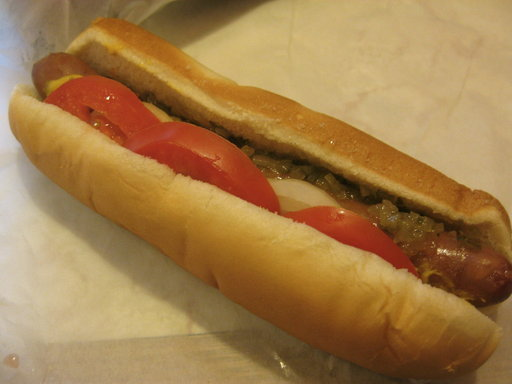
\includegraphics[width=.75\linewidth]{food1} 
    \caption{Hotdog} 
    \vspace{4ex}
  \end{minipage}%%
  \begin{minipage}[b]{0.25\linewidth}
    \centering
    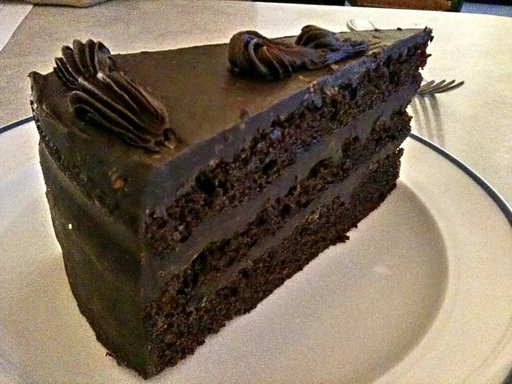
\includegraphics[width=.75\linewidth]{food2} 
    \caption{Chocolate Cake} 
  \label{fig:page2}
    \vspace{4ex}
  \end{minipage} 
  \begin{minipage}[b]{0.25\linewidth}
    \centering
    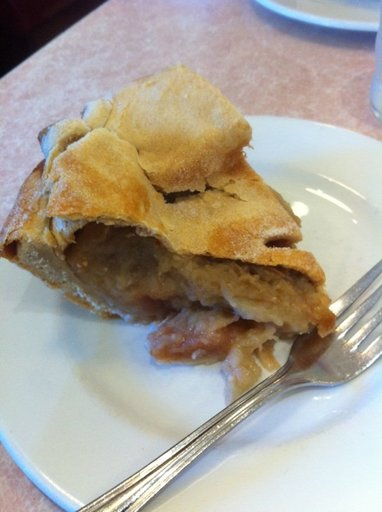
\includegraphics[width=.75\linewidth]{food3} 
    \caption{Apple Pie} 
    \vspace{4ex}
  \end{minipage}%% 
  \begin{minipage}[b]{0.25\linewidth}
    \centering
    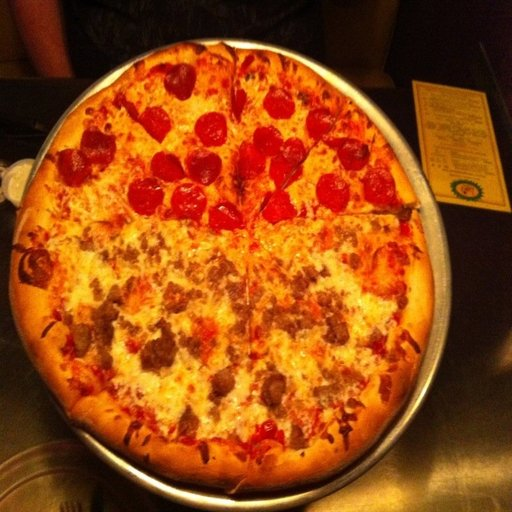
\includegraphics[width=.75\linewidth]{food4} 
    \caption{Pizza} 
    \vspace{4ex}
  \end{minipage} 
\end{figure}

\tocless\subsection{MNIST}
The MNIST dataset (created by \parencite{mnist}) consists of 70,000 hand written digits.
It is widely used in introductory CNN tutorials.
The dataset is split into 60,000 training images and 10,000 test images.
All the images are of the same dimensions.
Examples from the MNIST dataset can be seen in below.

\begin{figure}[h] 
  \label{mnistDataset} 
  \begin{minipage}[b]{0.25\linewidth}
    \centering
    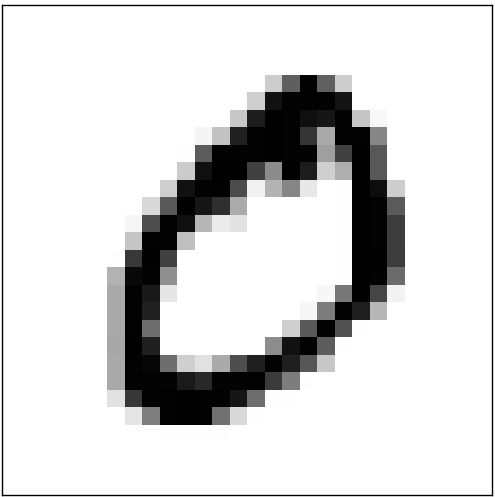
\includegraphics[width=.75\linewidth]{mnist0} 
    \caption{MNIST 0} 
    \vspace{4ex}
  \end{minipage}%%
  \begin{minipage}[b]{0.25\linewidth}
    \centering
    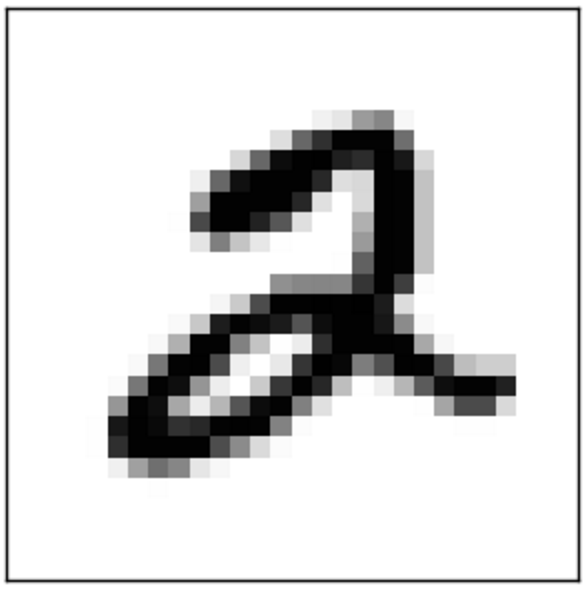
\includegraphics[width=.75\linewidth]{mnist2} 
    \caption{MNIST 2} 
  \label{fig:page2}
    \vspace{4ex}
  \end{minipage} 
  \begin{minipage}[b]{0.25\linewidth}
    \centering
    
\includegraphics[width=.75\linewidth]{mnist4} 
    \caption{MNIST 4} 
    \vspace{4ex}
  \end{minipage}%% 
  \begin{minipage}[b]{0.25\linewidth}
    \centering
    
\includegraphics[width=.75\linewidth]{mnist5} 
    \caption{MNIST 5} 
    \vspace{4ex}
  \end{minipage} 
\end{figure}

\tocless\subsection{CIFAR-10}
\parencite{cifar} created the CIFAR-10 dataset which consists of 10 classes.
Each of the 10 classes has 6,000 32x32 colour image associated and these are split between a 5,000 image training set and a 1,000 image test set.
There are five training batches and one test batch in the dataset.
The test set contains 1,000 randomly selected images from each class.
The training batches consist of random orderings of the remaining images.
Examples from the CIFAR-10 dataset can be seen below.

\begin{figure}[h] 
  \label{cifar10} 
  \begin{minipage}[b]{0.25\linewidth}
    \centering
    
\includegraphics[width=.75\linewidth]{cifar1} 
    \caption{CIFAR-10 Truck} 
    \vspace{4ex}
  \end{minipage}%%
  \begin{minipage}[b]{0.25\linewidth}
    \centering
    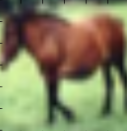
\includegraphics[width=.75\linewidth]{cifar2} 
    \caption{CIFAR-10 Horse} 
  \label{fig:page2}
    \vspace{4ex}
  \end{minipage} 
  \begin{minipage}[b]{0.25\linewidth}
    \centering
    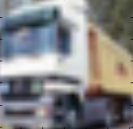
\includegraphics[width=.75\linewidth]{cifar3} 
    \caption{CIFAR-10 Boat} 
    \vspace{4ex}
  \end{minipage}%% 
  \begin{minipage}[b]{0.25\linewidth}
    \centering
    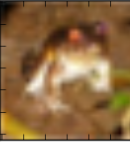
\includegraphics[width=.75\linewidth]{cifar4} 
    \caption{CIFAR-10 Frog} 
    \vspace{4ex}
  \end{minipage} 
\end{figure}

\section{Conclusion}
This chapter has covered a comprehensive survey of literature along with an overview of the underlying concepts to the approaches used in the literature.
This survey has covered the topics of using CNNs, SVMs and other methods for nutritional assessment.
Topics also covered include evaluating the output, object detection using CNNs, neural computing, an overview of CNNs and SVMs and an overview of the technologies used in this project.

From the literature review, there are many different approaches that have been promising in the area of using deep learning for nutritional assessment.
It has been decided to attempt to replicate the work carried out by \parencite{yanaiFood} with some modifications that will be outlined in the following chapters.
While this approach will be attempted, there are many viable options that can still be investigated for future work.


